\section*{Anhang: Vorbereitete Fragen}

\begin{frame}
  \only<1>{
  \begin{exampleblock}{Leitfrage}
    \begin{quotation}
      Die Art von Informationen, die ein Mensch mit einem Cochlea-Implantat beim Musikhören bekommt, ist so, als würde jemand am Klavier nicht mit einzelnen Fingern eine Melodie spielen, sondern mit seinen kompletten Unterarmen. Die einzelnen Elektroden der Cochlea-Implantate decken jeweils ein so breites Frequenzspektrum ab, dass sich Tonhöhen kaum unterscheiden lassen.
    \end{quotation}
  \end{exampleblock}}

  \only<2>{
  \begin{exampleblock}{Leitfrage}
    \begin{quotation}
      Die Art von Informationen, die ein Mensch mit einem \alert{Cochlea-Implantat} beim Musikhören bekommt, ist so, als würde jemand am Klavier nicht mit einzelnen Fingern eine Melodie spielen, sondern mit seinen kompletten Unterarmen. Die einzelnen Elektroden der Cochlea-Implantate decken jeweils ein so \alert{breites Frequenzspektrum} ab, dass sich Tonhöhen kaum unterscheiden lassen.
    \end{quotation}
  \end{exampleblock}}

\end{frame}

\subsection{Einstieg}
\begin{frame}
  \begin{figure}
    \centering
    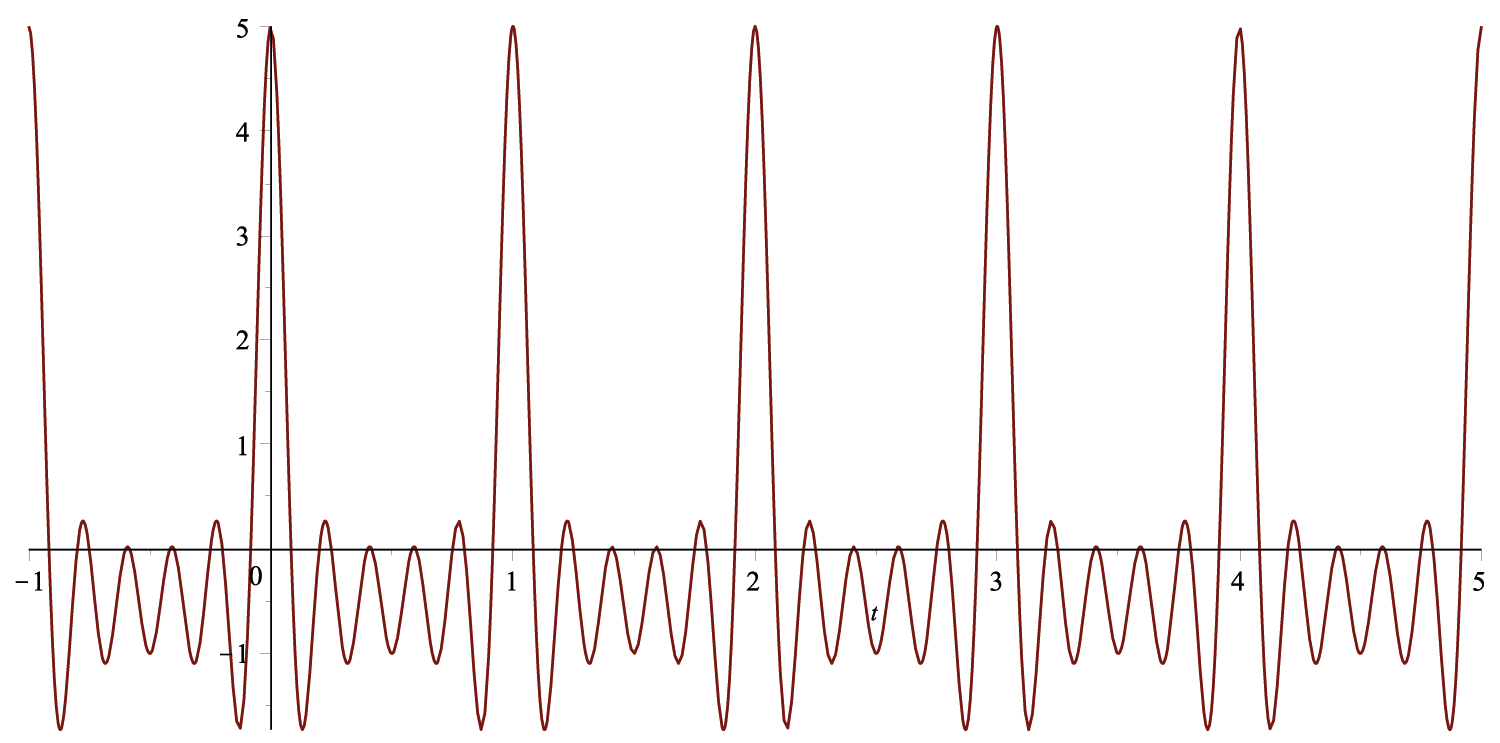
\includegraphics[width=\linewidth]{img/intro_harmonics}
    \caption{Auslenkungs-Zeit-Diagramm von Grund- und Oberschwingungen}
    \label{img:harmonics}
  \end{figure}
\end{frame}

\begin{frame}
  \begin{figure}
    \centering
    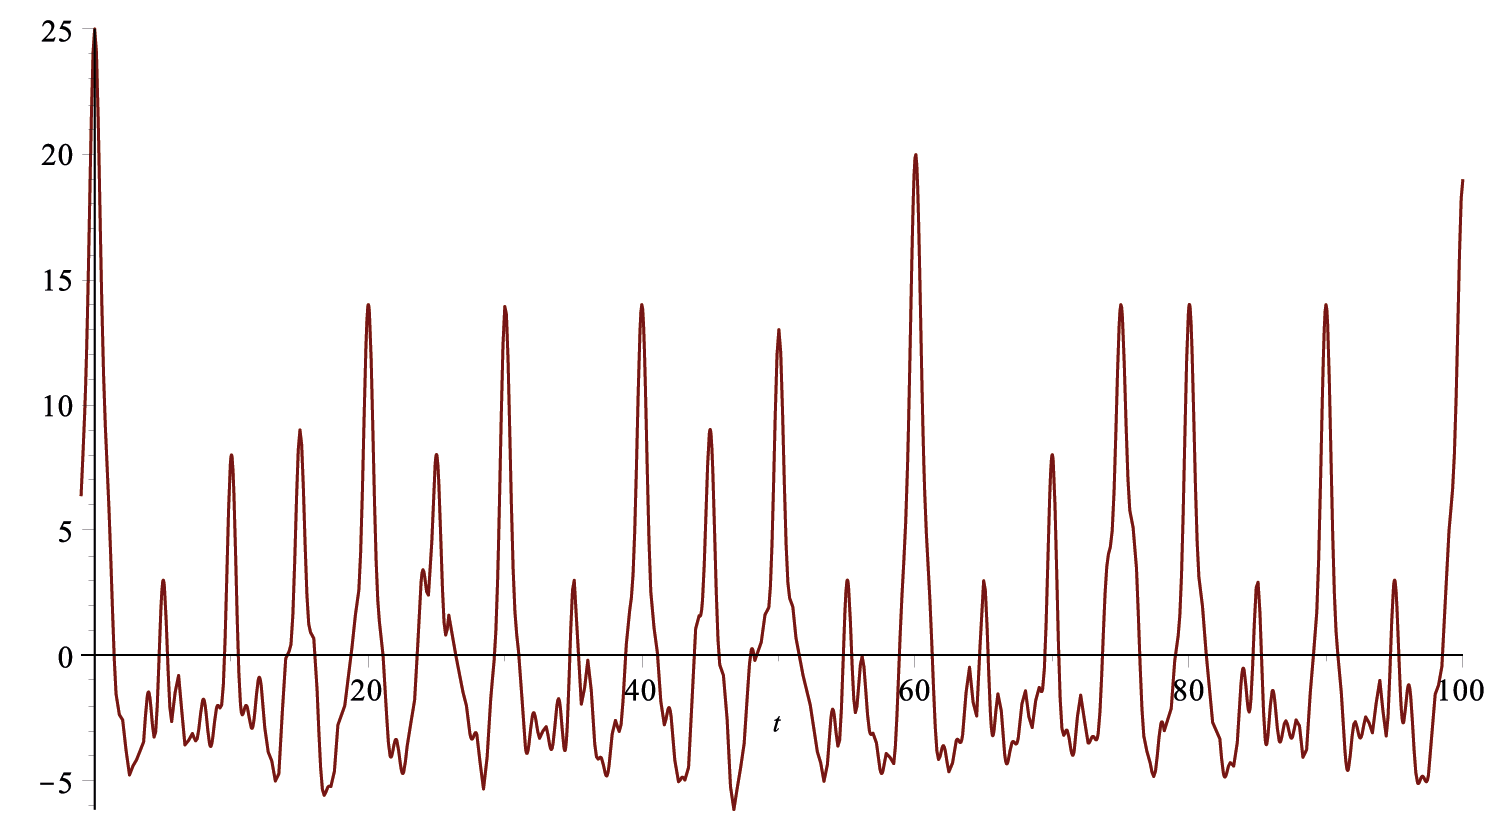
\includegraphics[width=\linewidth]{img/intro_interference}
    \caption{Auslenkungs-Zeit-Diagramm von verschiedenen Grund- und Oberschwingungen}
    \label{img:interference}
  \end{figure}
\end{frame}

\subsection{Mathematische Herleitung}
\begin{frame}
  \frametitle{Hilberträume}

  \begin{itemize}
    \item Vektorraum wird durch ein Skalarprodukt $ \langle f, g \rangle $ und Orthonormalbasen definiert
    \item \emph{Orthogonalität} bedeutet $\langle f, g \rangle = 0$
  \end{itemize}

  \begin{align*}
    \langle f, g \rangle = \int_{-\pi}^{\pi} f(x) \cdot g(x) \, dx
  \end{align*}
\end{frame}

\begin{frame}
  \frametitle{Orthonormalvektoren}

  \begin{align*}
    &\int_{-\pi}^{\pi} sin(k x) \, dx &&= 0 && \Rightarrow && sin(k x) \perp 1 \\
    &\int_{-\pi}^{\pi} cos(k x) \, dx &&= 0 && \Rightarrow && cos(k x) \perp 1 \\
    &\int_{-\pi}^{\pi} sin(k x)\cdot cos(m x) \, dx &&= 0 && \Rightarrow && sin(k x) \perp cos(m x) \\
    &\int_{-\pi}^{\pi} sin(k x)\cdot sin(m x) \, dx &&= \pi \cdot \delta_{m n} && \Rightarrow && sin(k x) \perp sin(m x), k \neq m \\
    &\int_{-\pi}^{\pi} cos(k x)\cdot cos(m x) \, dx &&= \pi \cdot \delta_{m n} && \Rightarrow && cos(k x) \perp cos(m x), k \neq m \\
    &\int_{-\pi}^{\pi} 1 \, dx &&= 2 \pi && \Rightarrow && 1 \not\perp 1
  \end{align*}
\end{frame}

\begin{frame}
  \frametitle{Fourieranalyse}

  \begin{align*}
    f(t) = \frac{a_0}{2} &+ a_1 \cdot cos(  t) + a_2 \cdot cos(2   t) + ... + a_n \cdot cos(n   t) \\ &+ b_1 \cdot sin( t) + b_2 \cdot sin(2  t) + ... + b_n \cdot sin(n  t)
   \end{align*}
   \begin{align*}
     \int_{-\pi}^{\pi} f(t) \cdot cos(n t) \, dx = &\int_{-\pi}^{\pi} \frac{a_0}{2} \cdot cos(n t) \,dx \\
      &+ a_n \int_{-\pi}^{\pi} cos(n  t) \cdot cos(n t) \, dx \\
      &+ b_n \int_{-\pi}^{\pi} sin(n  t) \cdot cos(n t) \, dx\\
      &= \pi \cdot a_n
    \end{align*}
\end{frame}
